\documentclass[11pt,aspectratio=43,ignorenonframetext,t]{beamer}
\usepackage{longtable}
% Uses fontspec - assumes compiled with LuaLaTeX or similar
% The above \documentclass is for making slides. If making handouts use:
%\documentclass[11pt,a4paper]{article} 
%\usepackage{beamerarticle}
%\setjobnamebeamerversion{main.beamer}

% See https://github.com/CASSON-LAB/uom_beamer_template
% for details on license, further useage information and similar
%%%%%%%%%%%%%%%%%% DOCUMENT SETUP %%%%%%%%%%%%%%%%%%

% Presentation settings
\mode<presentation>{
  \usetheme[framenumber,titleframestart=1]{UoM_alex}
  \usefonttheme{professionalfonts} % using non standard fonts for beamer
  \usefonttheme{serif}             % set font to Arial
  \usepackage{fontspec}
  \setmainfont[Ligatures=TeX]{Arial}
}

% Handout settings
\mode<article>{
  \usepackage{fullpage}                  % use full page
  \usepackage{fontspec}                  % set font to Arial
    \setmainfont[Ligatures=TeX]{Arial}
  \setlength{\parskip}{1.5\baselineskip} % correct beamer line spacings
  \setlength{\parindent}{0cm}
  \usepackage{enumitem}
    \setlist[itemize]{topsep=0pt}
  \definecolor{uomlinkblue}{HTML}{0071BC}
}


% Packages

% Configurando layout para mostrar codigos C++
\usepackage{listings}
\lstset{
  language=HTML,
  basicstyle=\ttfamily\small, 
  keywordstyle=\color{blue}, 
  stringstyle=\color{red}, 
  commentstyle=\color{red}, 
  extendedchars=true, 
  showspaces=false, 
  showstringspaces=false, 
  numbers=left,
  numberstyle=\tiny,
  breaklines=true, 
  backgroundcolor=\color{green!10},
  breakautoindent=true, 
  captionpos=b,
  xleftmargin=0pt,
}

\usepackage{graphicx}  % for graphics files
  \graphicspath{ {./fig/aula3} }
\usepackage{amsmath}   % assumes amsmath package installed
  \allowdisplaybreaks[1] % allow eqnarrays to break across pages
\usepackage{amssymb}   % assumes amsmath package installed 
\usepackage{hyperref} % add hyperlinks to document. Settings are for accessiblity
  \hypersetup{
    colorlinks=true,
    linkcolor=uomlinkblue,
    filecolor=uomlinkblue,      
    urlcolor=uomlinkblue,
	pdflang={en-GB},
}
\usepackage[document]{ragged2e} % left aligned text for accessibility
% experimental - does fundamentally work, if with quite a bit of effort
%\usepackage{axessibility} % LaTeX readable equations for accessibility
%  \tagpdfsetup{tabsorder=structure,uncompress,activate-all,interwordspace=true}
%  \pdfextension catalog{/Lang (en-GB)}
%  \RequirePackage{luacode}
%  \directlua{require("axessibility.lua")}
\usepackage{unicode-math} % unicode maths for accessibility
\usepackage{pdfcomment} % for alt text for accessibility
\usepackage{rotating}  % allow portrait figures and tables
\usepackage{subfigure} % allow matrices of figures
\usepackage{float}     % allows H option on floats to force here placement
\usepackage{multirow}  % allows merging of rows in tables
\usepackage{tabularx}  % allows fixed width tables
\usepackage{ctable}    % modifies \hline for use in table
\usepackage{bm}        % allow bold fonts in equations
\usepackage{pgf}       % allow graphics manipulation
\usepackage{media9}    % allow interactive flash files to be embedded
  \addmediapath{../media}
\usepackage{etoolbox}
  \makeatletter \preto{\@verbatim}{\topsep=0pt \partopsep=0pt} \makeatother  
  
% Custom commands
\newcommand{\matlab}{\emph{\sc{Matlab}}}
\newcommand{\maple}{\emph{\sc{Maple}}}
\newcommand{\simulink}{\emph{\sc{Simulink}}}
\newcommand{\dc}{d.c.}
\newcommand{\ac}{a.c.}
\newcommand{\rms}{RMS}
\newcommand{\wgn}{{\tt wgn}}
\newcommand{\sus}[1]{$^{\mbox{\scriptsize #1}}$}
\newcommand{\sub}[1]{$_{\mbox{\scriptsize #1}}$}
\newcommand{\chap}[1]{Chapter~\ref{#1}}
\newcommand{\sect}[1]{Section~\ref{#1}}
\newcommand{\fig}[1]{Fig.~\ref{#1}}
\newcommand{\tab}[1]{Table~\ref{#1}}
\newcommand{\equ}[1]{(\ref{#1})}
\newcommand{\appx}[1]{Appendix~\ref{#1}}
\newcommand{\degree}{\ensuremath{^\circ}}
\newcommand{\Vrms}{Vrms}
\newcommand{\Vpp}{V\sub{pp}}
\newcommand{\otoprule}{\midrule[\heavyrulewidth]}         
\newcolumntype{Z}{>{\centering\arraybackslash}X}  % tabularx centered columns 
\makeatletter \DeclareRobustCommand{\em}{\@nomath\em \if b\expandafter\@car\f@series\@nil \normalfont \else \bfseries \fi} \makeatother
\newcounter{example_number} % keep track of the example questions



%%%%%%%%%%%%%%%%%% FRONT MATTER %%%%%%%%%%%%%%%%%%
\title{Desenvolvimento de Software}
\subtitle{Atividades do bimestre 1}
\author{Prof. Me. Juliana Costa-Silva}
\begin{document}
%%%%%%%%%%%%%%%%%% TITLE SLIDE %%%%%%%%%%%%%%%%%%
\mode<presentation>{ \frame{\titlepage \label{slide:a}}} 
%\begin{figure}[!ht] 
%\fbox{\includeslide[width=\textwidth]{slide:a}} \end{figure}



%%%%%%%%%%%%%%%%%% NEW SLIDE %%%%%%%%%%%%%%%%%%
\clearpage 
\mode<presentation>{\begin{frame}{Na aula de hoje...}
  \setbeamertemplate{section in toc}[sections numbered]
  \tableofcontents[hideallsubsections]
\end{frame}}
%---------------------------------------------------------------% Fonte: https://www.ic.unicamp.br/~santanch/teaching/oop/2015-1/exercicios.html/
% Fonte[2]: http://www.ic.uff.br/~leomurta/courses/2016.1/poo/lista.pdf
\section{Atividades - Estruturada}
\mode<presentation>{\begin{frame}{Atividade 1}
Um trabalhador autônomo deseja controlar suas fincanças, comprou um microcomputador para controlar o rendimento diário de seu trabalho. 
\begin{itemize}
    \item Toda vez que ele vende um valor maior que o estabelecido pelo regulamento de MEI do estado onde vive (500,00 R\$ dia) deve pagar um multa de R\$ 0,10 a cada  Real excedente.
    \item Este trabalhador precisa que você faça um programa em Java que leia o valor de todas as vendas do mês e verifique se há excesso (vendeu mais de 500,00 por dia). 
    \item Se houver excesso, gravar na variável E (Excesso) e na variável M o valor da multa que o Trabalhador deverá pagar. 
    \item Caso contrário mostrar tais variáveis com o conteúdo ZERO.
\end{itemize} 
\end{frame}}

%----------------------------------------------------------------------------
\mode<presentation>{\begin{frame}{Atividade 2}
Uma empresa de vendas precisa implementar a rotina de cobrança com a seguinte regra:
\begin{itemize}
    \item Os boletos atrasados devem receber uma multa de 5\% no primeiro dia de atraso, mais os juros;
    \item O valor do boleto deve ser recalculado a cada dia com juros de 1\% por dia de atraso (juros sobre juros);
    \item Desenvolva um programa em Java, que dado o valor original do boleto, e os dias de atraso calcule o valor total a ser pago;
\end{itemize}
\textcolor{gray}{Exemplo: Um boleto no valor de R\$ 259,90 com 2 dias de atraso deve ser recalculado em R\$ 278,38 }
 
\end{frame}}
%------------------------------------------------
\mode<presentation>{\begin{frame}{Atividade 3}
    A empresa de saneamento de uma cidade que controla o índice de poluição da água e mantém 3 grupos de indústrias que são altamente poluentes para o meio ambiente.
    \begin{itemize}
        \item O índice de poluição aceitável varia de 0,06 até 0,16. 
        \item Se o índice sobe para 0,25 as indústrias do 1º grupo são intimadas a reduzirem em 50\% suas atividades;
        \item Se o índice crescer para 0,4 as industrias do 1º e 2º grupo são intimadas a suspenderem suas atividades.
        \item Se o índice atingir 0,5 todos os grupos devem ser notificados a paralisarem suas atividades. 
        \item Desenvolva um programa em Java que leia o índice de poluição medido e emita a notificação adequada aos diferentes grupos de empresas.
    \end{itemize}
\end{frame}}

%----------------------------------------------------------------------
\mode<presentation>{\begin{frame}{Atividade 4}
  Foi feita uma pesquisa entre os habitantes de uma cidade. Foram coletados os dados de idade, gênero (M/F) e renda. Faça um algoritmo contenha um menu onde seja possível registrar, os dados de cada habitante e, ainda consultar as seguintes informações:
  \begin{enumerate}
      \item A média de salário do grupo;
      \item Maior e menor idade do grupo;
      \item Quantidade de habitantes do gênero masculino com salário até R\$ 1000,00;
      \item Quantidade de habitantes do gênero feminino;
  \end{enumerate}
\end{frame}}
%-----------------------------------------------------
\mode<presentation>{\begin{frame}{Atividade 5}
\tiny{
Um banco realiza empréstimos nas seguintes condições: 
\begin{itemize}
    \item são tomados  X reais emprestados; 
    \item N reais serão pagos cada mês até que o empréstimo seja quitado;
    \item parte do pagamento mensal serão juros, calculados como j por cento do saldo corrente;
    \item o restante será aplicado no pagamento da dívida;
\end{itemize}

Escreva um programa que leia estes três valores: X, N, j e determine: 
\\
Para cada mês:\\
\textbf{a)} valor em dinheiro dos juros pagos; \\
\textbf{b)} valor em dinheiro aplicada no pagamento da dívida;\\
\textbf{c)} valor acumulado de juros já pagos; \\
\textbf{d)} valor ainda por pagar do empréstimo no fim de cada mês;\\
No final do programa:\\ 
\textbf{e)} número de meses necessários para pagar o empréstimo; \\
\textbf{f)} quantidade da última prestação.\\
}

\end{frame}}
%------------------------------------------
\mode<presentation>{ \begin{frame}{Atividade 6}
    Escreva um programa que determine se uma cadeia de caracteres é um palíndromo ou não. Um palíndromo é uma cadeia que é igual à sua inversa.\\
    
    \textbf{Exemplos:} \\
    ASA = ASA (inverso) -> é um PALÍNDROMO \\
    JOAO <> OAOJ (inverso) -> não é um PALÍNDROMO\\
    343 = 343 (inverso) ->é um PALÍNDROMO
\end{frame}}
%------------------------------------------
\mode<presentation>{ \begin{frame}{Atividade 7}
    Escreva uma função que receba como parâmetro um número inteiro relativo a um mês do ano e retorne uma string com o nome deste mês por extenso. Resolva o problema de suas maneiras:
    \begin{enumerate}
        \item sem um vetor, através de uma estrutura switch/case;
        \item com um vetor.
    \end{enumerate}
\end{frame}}
%---------------------------------------------------------------
\mode<presentation>{\begin{frame}{Atividade 8}
\small
\textbf{5.} Um quadrado mágico é uma matriz quadrada em que a soma das suas linhas é igual a soma das sua colunas e que também é igual a soma da diagonal principal e da diagonal secundária. A matriz abaixo é um exemplo de quadrado mágico, pois a somatória, em todos os casos, é igual a 15.

\begin{center} 
   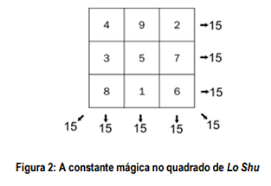
\includegraphics[height=0.2\paperheight]{fig/aula3/quadrado_magico.png} \\
 \end{center}
 Faça um código Java que receba uma dimensão N de uma matriz $A_{nxn}$, seguido dos respectivos valores da matriz (preenchendo a matriz da linha 0 até N, da esquerda para a direta: \textit{coluna 0 até N}), verificar se a matriz é um quadrado mágico (Imprima: “quadrado magico” caso seja e “quadrado NÃO magico” caso não seja).
 \textit{Obrigatório o uso de laço de repetição e arrays}
\end{frame}}
%-------------------------------------------------------------
\section{Atividades - Orientação a Objetos}
\mode<presentation>{\begin{frame}{Atividade O.O. [1]} % OO
  Uma empresa deseja otimizar o estoque de produtos, evitando a compra em excesso e/ou a falta no estoque. Elabore um programa Java para verificar que produtos precisam ser comprados e a quantidade a ser adquirida, com base nas seguintes informações:
  \begin{itemize}
      \item Cada produto em as seguintes informações: Código do produto, Quantidade Mínima, Quantidade Máxima e a quantidade em estoque;
      \item Um produto somente deverá ser comprado quando: a quantidade em estoque for menor ou igual a quantidade mínima;
      \item Ao final da execução exiba: Código do Produto e Quantidade a Comprar;
  \end{itemize}
\end{frame}}
%----------------------------------------------------------------------
\mode<presentation>{\begin{frame}{Atividade O.O. [2]}
\small
  Considere a seguinte classe, cujo método respostaQuestao recebe como parâmetro o número de uma pergunta e retorna a sua resposta correta, com base em um gabarito.
\begin{center}
  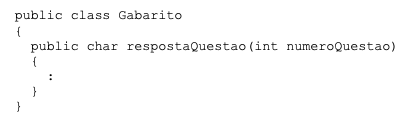
\includegraphics[height=0.3\paperheight]{fig/atv_bim1/atividade_6.png} \\
 \end{center}

\end{frame}}
%----------------------------------------------------------------------
\mode<presentation>{\begin{frame}{Atividade O.O. [continuação 2]}
\tiny{
\begin{itemize}
    \item Escreva uma classe classe \textbf{Avaliacao} em que cada objeto representa uma prova feita por um aluno;
     \item Esta avaliação possui 12 questões de múltipla escolha (letras A a E). As 10 primeiras questões valem 0,5 ponto e as 5 últimas questões valem 1 ponto;
    \item A classe \textbf{Avaliacao} deverá controlar as questões respondidas pelo aluno. Para isto, a classe deve implementar os métodos:
     \item \textbf{construtor da classe} recebe como parâmetro um objeto da classe Gabarito contendo o gabarito da prova;
     \item \textbf{respostaAluno} recebe como parâmetro a resposta dada pelo aluno a uma questão; este método não recebe entre os parâmetros o número da questão, ele mesmo deve estabelecer um controle interno para que as questões sejam inseridas em sequência, ou seja, a 1\textsuperscript{a} vez que o método é chamado, insere a 1\textsuperscript{a} questão, a 2\textsuperscript{a}, insere a 2\textsuperscript{a} questão, e assim por diante;
     \item \textbf{acertos} retorna a quantidade de questões que o aluno acertou;
     \item \textbf{nota} retorna a nota que o aluno tirou na prova;
     \item \textbf{maior} recebe como parâmetro um outro objeto da classe Prova e retorna a nota do aluno que acertou mais questões; se houver empate, retorna a maior nota; se houver empate novamente, retorna a nota do aluno representado no objeto corrente;
\end{itemize}}
\end{frame}}
%-----------------------------------------------------
\mode<presentation>{\begin{frame}{Atividade O.O. [3]}
\tiny{
  Escreva uma classe em que cada objeto representa uma viagem que acontece em determinada data e em determinado horário. Cada viagem possui no máximo 43 passageiros, e a classe permite controlar a ocupação das vagas. A classe deve ter os seguintes métodos:
  
\begin{table}[]
\begin{tabular}{|l|l|}
\hline
\textbf{método} & \textbf{descrição} \\ \hline
construtor & \begin{tabular}[c]{@{}l@{}}configura os dados da viagem (recebidos como \\ parâmetro): número da viagem,  data (para \\ armazenar a data utilize um objeto da classe \\ Date);\end{tabular} \\ \hline
proximoLivre & retorna o número da próxima cadeira livre \\ \hline
verifica & \begin{tabular}[c]{@{}l@{}}verifica se o número da cadeira recebido como \\ parâmetro está ocupada\end{tabular} \\ \hline
ocupa & \begin{tabular}[c]{@{}l@{}}ocupa determinada cadeira do viagem, cujo \\ número é recebido como parâmetro, \\ e retorna  verdadeiro se a cadeira ainda não \\ estiver ocupada (operação foi bem \\ sucedida) e falso  caso contrário\end{tabular} \\ \hline
vagas & \begin{tabular}[c]{@{}l@{}}retorna o número de cadeiras vagas disponíveis \\ (não ocupadas) na viagem.\end{tabular} \\ \hline
getViagem & retorna o número da viagem \\ \hline
getData & retorna a data da viagem (na forma de objeto) \\ \hline
clone & \begin{tabular}[c]{@{}l@{}}o objeto clona a si próprio, para isto, ele cria \\ um novo objeto da mesma classe \\ e faz uma  cópia dos valores de seus atributos\end{tabular} \\ \hline
\end{tabular}
\end{table}}
\end{frame}}

%------------------------------
\section{Leitura recomendada}
\mode<presentation>{
\begin{frame}{Leitura complementar [1]}
 Para mais informações sobre Java, leia:\\
 \begin{columns}
   \begin{column}{0.4\textwidth}
     Capítulo 1 a 7:
	   Livro: Java Como programar (Deitel e Deitel, 2017) \\
    \cite{deitel2017java}
   \end{column}
   \begin{column}{0.3\textwidth}
    \begin{center}
  
\includegraphics[height=0.5\paperheight]{fig/aula1/deitel2017java.png} 
 \end{center}
   \end{column}
 \end{columns}
 \textcolor{red}{DISPONÍVEL NA BIBLIOTECA VIRTUAL}
\end{frame}}
%-----------------------------------------------------
\mode<presentation>{
\begin{frame}{Leitura complementar [2]}
 Para mais informações sobre Java, leia:\\
 \begin{columns}
   \begin{column}{0.4\textwidth}
     Capítulo 1 a 5:
	Livro: Core Java (Horstman, 2013) \\
        \cite{horstmann2013core}
   \end{column}
   \begin{column}{0.3\textwidth}
    \begin{center}
  
\includegraphics[height=0.5\paperheight]{fig/horstman2013.png} \\
 \end{center}
   \end{column}
 \end{columns}
 \textcolor{red}{DISPONÍVEL NA BIBLIOTECA VIRTUAL}
\end{frame}}

 %----------------------------------------------------------------------------
 
 \mode<presentation>{\begin{frame}{Referências}%[allowframebreaks]
 \small
 \begin{center}
 	\bibliographystyle{apalike}
	 \bibliography{ref_aula_progI}
 \end{center}
 \end{frame}}

\begin{figure}[!ht] \fbox{\includeslide[width=\textwidth]{slide:z}} \end{figure}
Text for notes goes here. 
\begin{itemize}
  \item List 1. 
  \item List 2. 
\end{itemize}


%%%%%%%%%%%%%%%%%% END MATTER %%%%%%%%%%%%%%%%%%
\end{document}